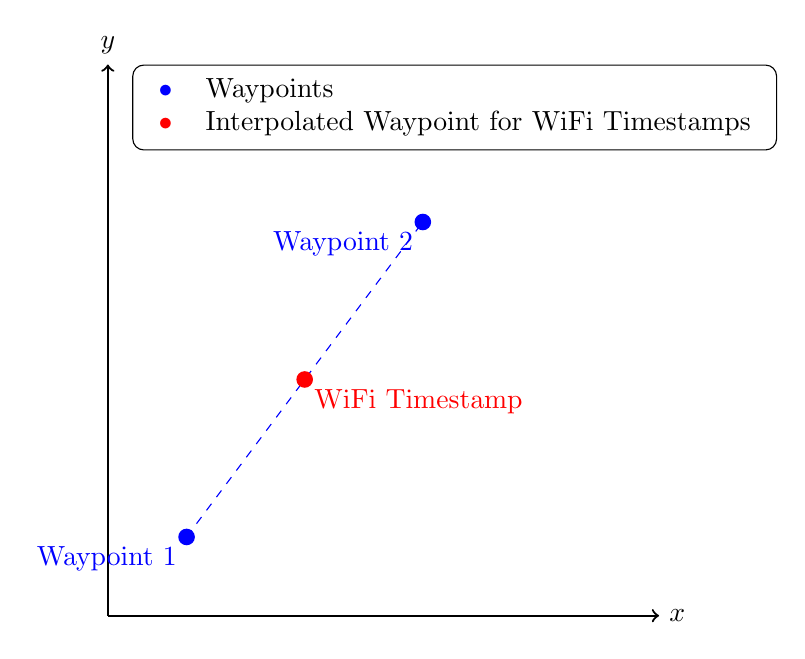
\begin{tikzpicture}
    % Axis
    \draw[->, thick] (0,0) -- (7,0) node[right] {$x$};
    \draw[->, thick] (0,0) -- (0,7) node[above] {$y$};

    % Given Waypoints (e.g., from the waypoints data)
    \fill[blue] (1,1) circle (3pt) node[below left] {Waypoint 1};
    \fill[blue] (4,5) circle (3pt) node[below left] {Waypoint 2};
    \draw[dashed, blue] (1,1) -- (4,5);

    % Interpolated Points (e.g., for wifi_timestamps)
    \fill[red] (2.5,3) circle (3pt) node[below right] {WiFi Timestamp};

    % Legend
    \node[draw, rectangle, rounded corners, fill=white, anchor=north east] at (8.5,7) {
        \begin{tabular}{c l}
        \color{blue} $\bullet$ & Waypoints \\
        \color{red} $\bullet$ & Interpolated Waypoint for WiFi Timestamps \\
        \end{tabular}
    };
\end{tikzpicture}